%%!TEX encoding = UTF-8 Unicode 
\documentclass[oneside,a4paper]{report}

% Use utf-8 encoding for foreign characters
\usepackage[utf8]{inputenc}

% Setup for fullpage use
\usepackage{fullpage}
\usepackage[usenames,dvipsnames]{color}
%\usepackage{subfigure}
% \usepackage{boxedminipage}
\usepackage{listings}
\usepackage{booktabs}
\usepackage{setspace}

\linespread{1.6}

\lstdefinelanguage[ARM]{Assembler}%
  {morekeywords=[1]{.text,.globl,.align},%
  morekeywords=[2]{add,beq,bge,blt,bne,cmp,ldr,mov,mul,pop,push,%
    subs,vadd,vld1,vldm,vmov,vmul,vpadd,vpop,vpush},%
   morekeywords=[3]{f32,s32,i32},%
   keywordsprefix=.,%
   sensitive,%
   morecomment=[l]//,% nonstandard
   moredelim=*[directive]\#,%
   moredirectives={define,elif,else,endif,error,if,ifdef,ifndef,line,%
      include,pragma,undef,warning}%
  }[keywords,comments,directives]

\lstset{
  numbers=left,
  numberstyle=\tiny,
  numbersep=10pt,
  basicstyle=\small\ttfamily,
  keywordstyle=[1]\color{RedOrange},
  keywordstyle=[2]\color{RoyalBlue},
  keywordstyle=[3]\color{Mulberry},
  identifierstyle=,
  commentstyle=\color{OliveGreen},
  stringstyle=\ttfamily,
  directivestyle=\color{OliveGreen},
  showstringspaces=false
}

% This is now the recommended way for checking for PDFLaTeX:
\usepackage{ifpdf}

%\newif\ifpdf
%\ifx\pdfoutput\undefined
%\pdffalse % we are not running PDFLaTeX
%\else
%\pdfoutput=1 % we are running PDFLaTeX
%\pdftrue
%\fi

\ifpdf
\usepackage[pdftex]{graphicx}
\else
\usepackage{graphicx}
\fi

\usepackage[colorlinks=true,citecolor=OrangeRed,urlcolor=NavyBlue,linkcolor=ForestGreen]{hyperref}
\usepackage[all]{hypcap}

\title{ \textbf{ARM Cortex-A8} \\ \large{4810-1164 Modern Computer Architectures and System Software}}
\author{ \textbf{Daniel Heffernan} \\ Creative Informatics (M1) -- 48-116625 }

\begin{document}

\ifpdf
\DeclareGraphicsExtensions{.pdf, .jpg, .tif}
\else
\DeclareGraphicsExtensions{.eps, .jpg}
\fi

\maketitle

\chapter{Introduction}

It is very popular recently, and its popularity is marked by its use by Apple as the CPU in the Apple A4 SoC (System on Chip), which powers Apple's iPad and iPhone 4. It is also notable for being the first implementation of the ARMv7 instruction set architecture which includes NEON \cite{Gris}, the \emph{single instruction, multiple data} (SIMD) unit which implements floating point (VFPv3) and SIMD (Advanced SIMD) instruction sets, and for operating at speeds of up to 1GHz in very low-power environments (sub-1W, and often around 300mW) \cite{Williamson}.

There are three Cortex series: Cortex-A, Cortex-R and Cortex-M. They are so named because of each series' ARMv7 instruction set profile. ARMv7-A is one of three available profiles of ARMv7 \cite[p. A1-4]{ARMRef}, and is used in the Cortex-A series. Cortex-R uses ARMv7-R, which is a real-time variant which uses a \emph{Protected Memory System Architecture} (PMSA) instead of ARMv7-A's \emph{Virtual Memory System Architecture} (VMSA). The Cortex-M series processors use the ARMv7-M profile, which is a microcontroller variant of ARMv7.

\begin{figure}[htbp]
	\centering
	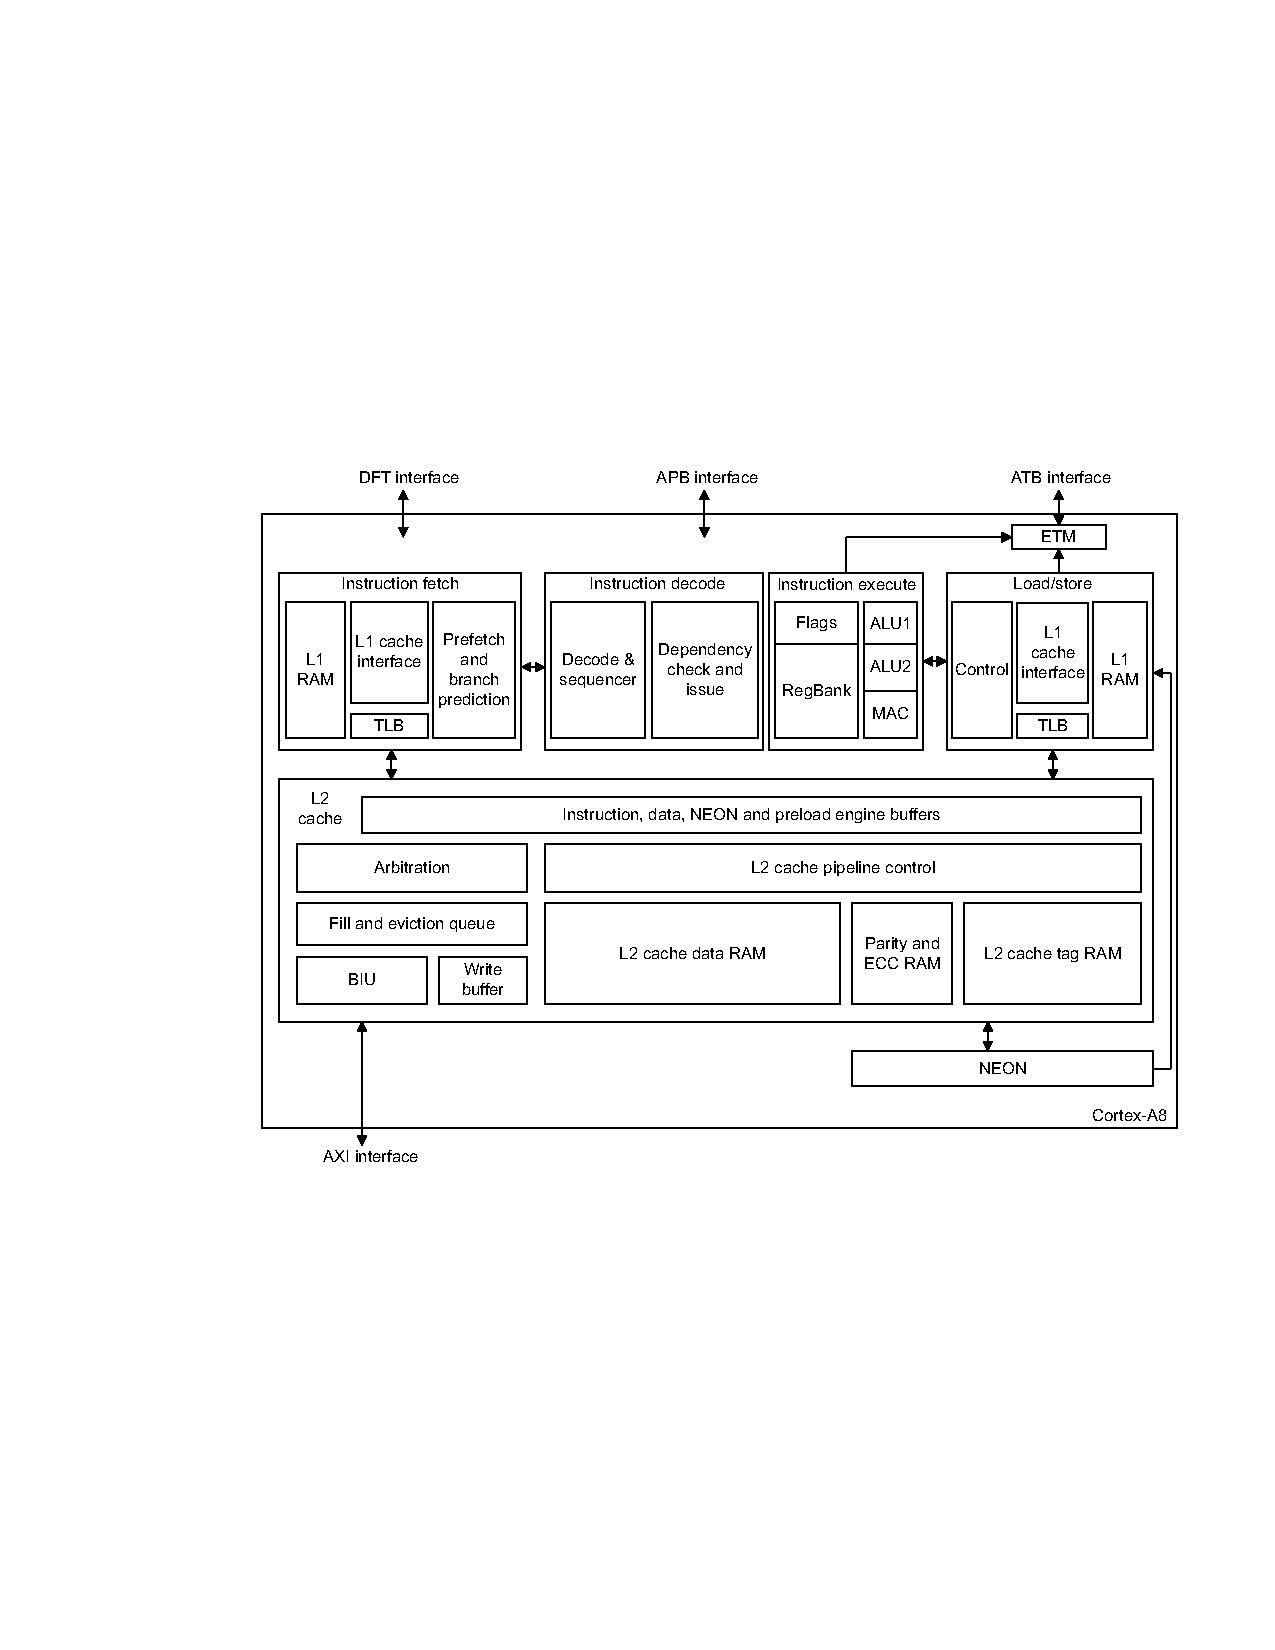
\includegraphics[width=1.0\textwidth]{./fig/CortexA8.pdf}
	\caption{Overview of the Cortex-A8 architecture from \cite[p. 1-4]{A8Ref}.}
	\label{fig:cortexa8}
\end{figure}

\chapter{Main Features}

ARM is a \emph{reduced instruction set computer} (RISC) architecture. It is a load/store architecture, meaning that its operations are performed on register contents, which are loaded from memory, and then stored back to memory; it does not perform operations directly on memory contents. It performs integer operations in a 13-stage pipeline, and floating point operations in a 10-stage NEON pipeline. The full pipeline is illustrated in Figure~\ref{fig:pipeline}.

The Cortex-A8 is a in-order, dual-issue, superscalar microprocessor core that supports the following instruction sets:
\begin{description}
	\item[ARM] is a 32-bit instruction set which includes some interesting features such as conditional execution of almost all instructions, execution of shift/rotate operations with ALU operations in the same instruction, and 2-word (64-bit) SIMD operations.
	
	\item[Thumb-2] is a variable-sized instruction set. Thumb is a 16-bit instruction subset of the ARM instruction set, created with the goal to increase code density. However, it reduced the number of available instructions so much that performance decreased, so Thumb-2 was created as a variable 16/32-bit instruction set aiming to provide ``Thumb code density at ARM performance'' \cite[p. 5]{Gris}.
	
	\item[VFPv3] (\emph{Vector Floating Point v3}) is a floating point instruction set, which is executed in the NEON unit. It supports single-word and double-word operations in its 16 double-word registers.
	
	\item[Advanced SIMD] is a SIMD instruction set that works together with VFPv3 in the NEON unit. It shares the VFPv3 registers, but can also address them as quad-word (128-bit) registers. Advanced SIMD operations can execute double-word or quad-word operands in parallel.
\end{description}

\begin{figure}[htbp]
	\centering
	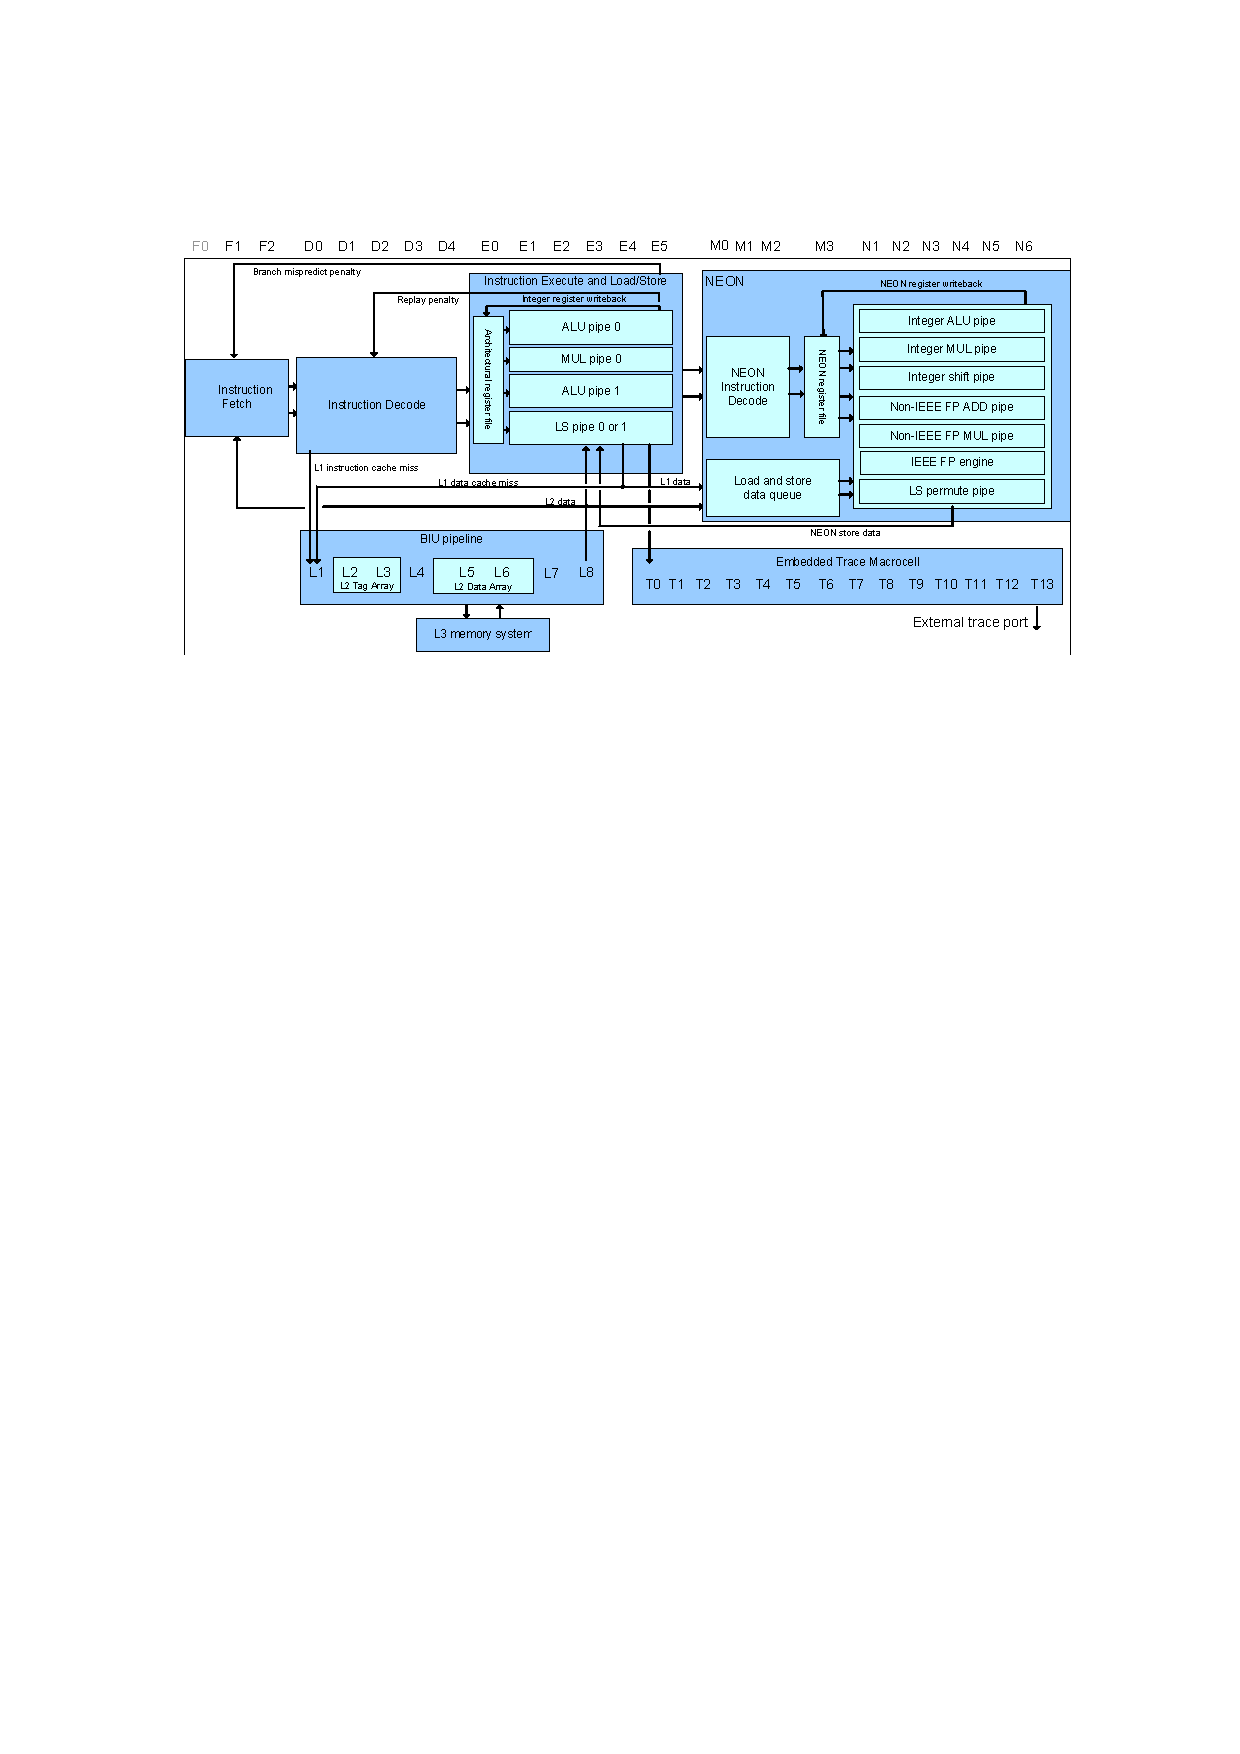
\includegraphics[width=1.0\textwidth]{./fig/Pipeline.pdf}
	\caption{Cortex-A8 full pipeline from \cite[p. 3]{Williamson}.}
	\label{fig:pipeline}
\end{figure}

\chapter{Registers}

ARM Cortex-A8 contains 16 user registers are 32 bits long. However, load and store operations are not limited to word-sized data, and these operations can be performed with bytes, half-words, words and double-words. There are also load and store operations that support two or more words of data, so it is possible to fill all registers with a single load.

The processor has 40 registers \cite[p. 2-18]{A8Ref}. This includes 33 general-purpose registers and 7 \emph{saved program status registers} (SPSRs). The format of a SPSR on a Cortex-A8 processor is illustrated in Figure~\ref{fig:cpsr}. In user-mode 16 data registers and 2 status registers are accessible, and these are described in Table~\ref{tab:registers}. Though 16 registers are available, many of these are reserved. r13, r14 and r15 are used for the stack pointer, link register and program counter, respectively. On iOS r7 is also reserved for use as the frame pointer.

\begin{figure}[htb]
	\centering
	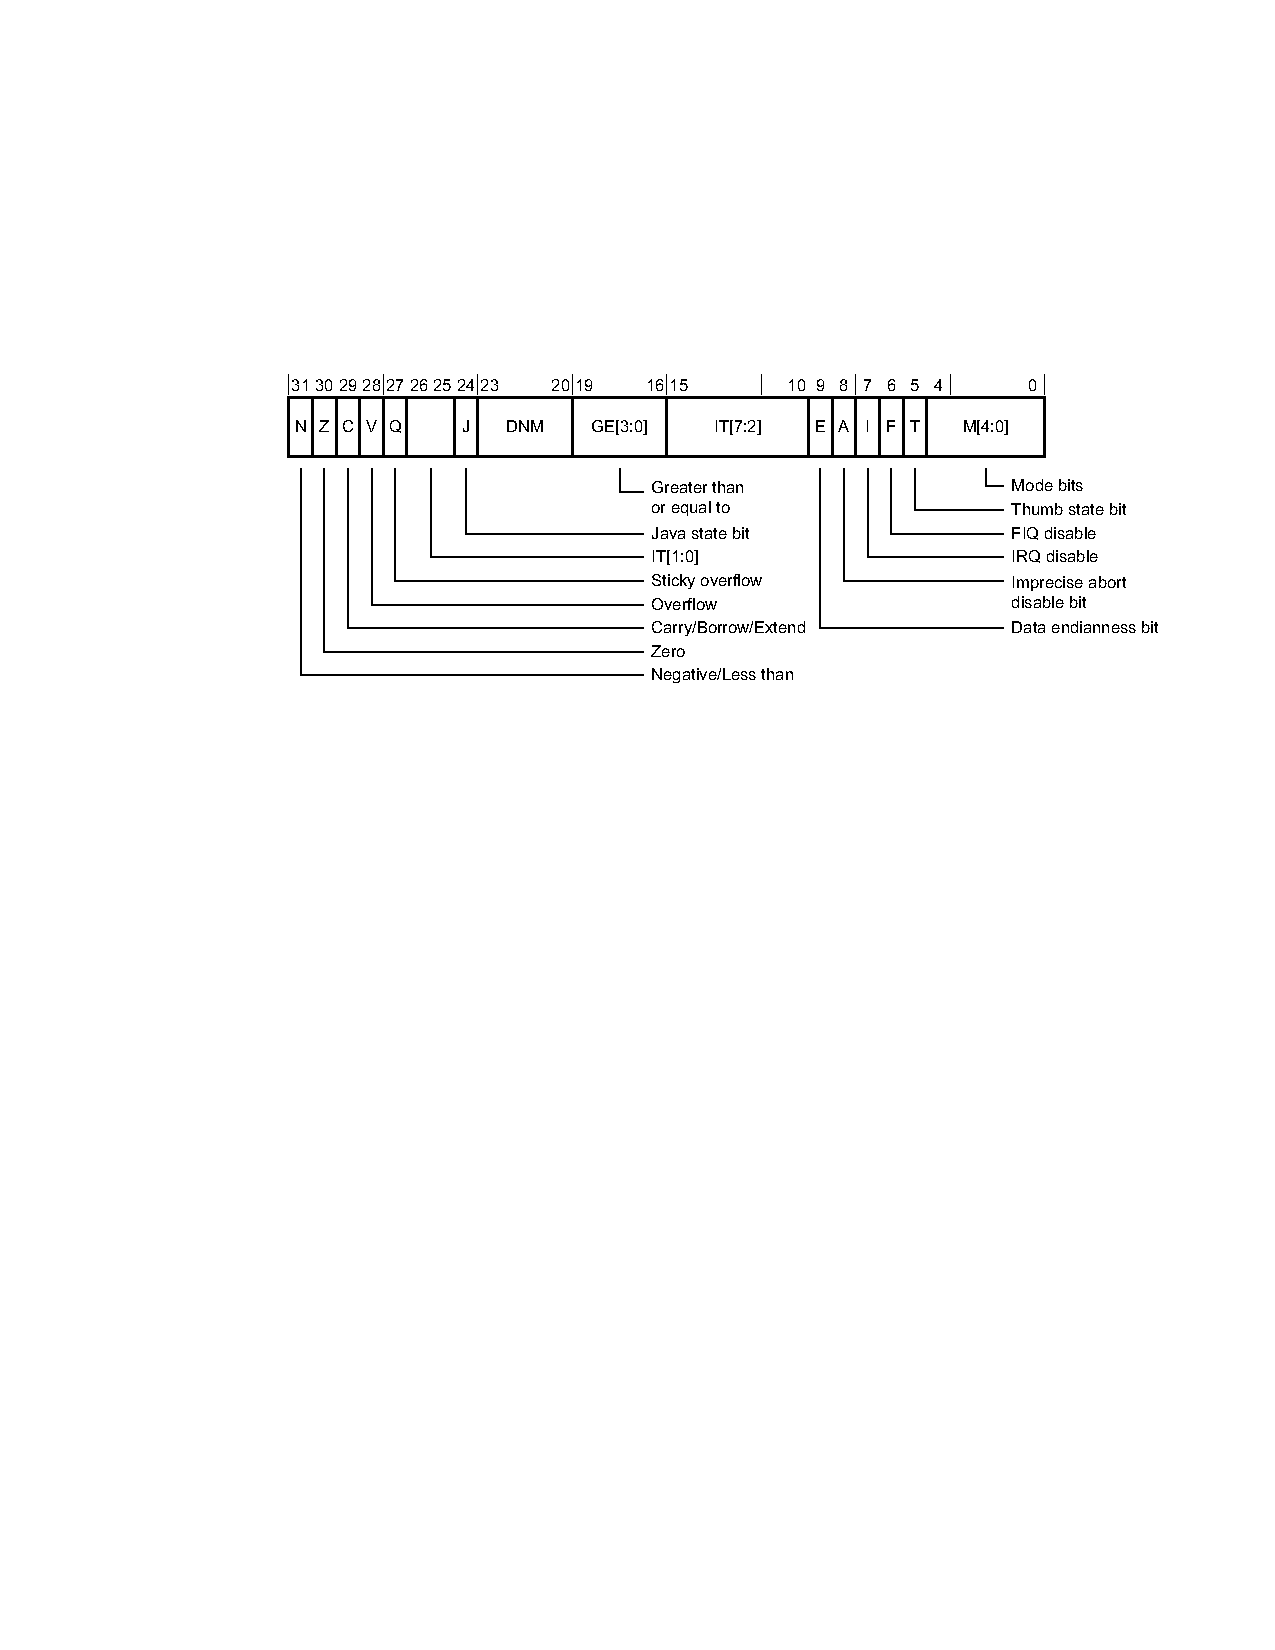
\includegraphics[width=1.0\textwidth]{./fig/CPSR.pdf}
	\caption{Program status register from \cite[p. 2-21]{A8Ref}.}
	\label{fig:cpsr}
\end{figure}

The NEON unit also has its own registers for use in VFP and NEON operations. There are 8 128-bit (quad-word) registers available. These can also be addressed as 16 double-word registers or 32 single-word registers. This is illustrated in Table~\ref{tab:registers}.

\begin{table}[p]
	\centering
	\singlespacing
		\begin{tabular}{lllllll}
		\toprule
		Type						&	\multicolumn{3}{l}{Name}	&	Preserved	&	Notes						\\
		\midrule
	 	General-purpose register	&	\multicolumn{3}{l}{R0}		&	No			&	Argument/result/scratch 1   \\
							 		&	\multicolumn{3}{l}{R1}		&	No			&	Argument/result/scratch 2   \\
							 		&	\multicolumn{3}{l}{R2}		&	No			&	Argument/scratch 3			\\
							 		&	\multicolumn{3}{l}{R3}		&	No			&	Argument/scratch 4			\\
							 		&	\multicolumn{3}{l}{R4}		&	Yes			&	Variable register 1			\\
							 		&	\multicolumn{3}{l}{R5}		&	Yes			&	Variable register 2			\\
							 		&	\multicolumn{3}{l}{R6}		&	Yes			&	Variable register 3			\\
							 		&	\multicolumn{3}{l}{R7}		&	Yes			&	Variable register 4 / Frame pointer on iOS	\\
							 		&	\multicolumn{3}{l}{R8}		&	Yes			&	Variable register 5			\\
							 		&	\multicolumn{3}{l}{R9}		&	Special		&	Platform register			\\
							 		&	\multicolumn{3}{l}{R10}		&	Yes			&	Variable register 7			\\
							 		&	\multicolumn{3}{l}{R11}		&	Yes			&	Variable register 8			\\
							 		&	\multicolumn{3}{l}{R12}		&	No			&	The Intra-Procedure-call scratch register (IP)	\\
							 		&	\multicolumn{3}{l}{R13}		&	Special		&	Stack pointer (SP)	 		\\
							 		&	\multicolumn{3}{l}{R14}		&	Special		&	Link register (LR)	 		\\
							 		&	\multicolumn{3}{l}{R15}		&	Special		&	Program counter (PC) 		\\
		Program status register		&	\multicolumn{3}{l}{CPSR}	&	Special		&						 		\\
		NEON register				&	Q0	&	D0	&	S0			&	No			&	  		\\
									&		&		&	S1			&	No			&	  		\\
									&		&	D1	&	S2			&	No			&	  		\\
									&		&		&	S3			&	No			&	  		\\
									&	Q1	&	D2	&	S4			&	No			&	  		\\
									&		&		&	S5			&	No			&	  		\\
									&		&	D3	&	S6			&	No			&	  		\\
									&		&		&	S7			&	No			&	  		\\
									&	Q2	&	D4	&	S8			&	No			&	  		\\
									&		&		&	S9			&	No			&	  		\\
									&		&	D5	&	S10			&	No			&	  		\\
									&		&		&	S11			&	No			&	  		\\
									&	Q3	&	D6	&	S12			&	No			&	  		\\
									&		&		&	S13			&	No			&	  		\\
									&		&	D7	&	S14			&	No			&	  		\\
									&		&		&	S15			&	No			&	  		\\
									&	Q4	&	D8	&	S16			&	Yes			&	  		\\
									&		&		&	S17			&	Yes			&	  		\\
									&		&	D9	&	S18			&	Yes			&	  		\\
									&		&		&	S19			&	Yes			&	  		\\
									&	Q5	&	D10	&	S20			&	Yes			&	  		\\
									&		&		&	S21			&	Yes			&	  		\\
									&		&	D11	&	S22			&	Yes			&	  		\\
									&		&		&	S23			&	Yes			&	  		\\
									&	Q6	&	D12	&	S24			&	Yes			&	  		\\
									&		&		&	S25			&	Yes			&	  		\\
									&		&	D13	&	S26			&	Yes			&	  		\\
									&		&		&	S27			&	Yes			&	  		\\
									&	Q7	&	D14	&	S28			&	Yes			&	  		\\
									&		&		&	S29			&	Yes			&	  		\\
									&		&	D15	&	S30			&	Yes			&	  		\\
									&		&		&	S31			&	Yes			&	  		\\
		VFP status register			&	\multicolumn{3}{l}{FPSCR}	&	Special		&						 		\\
		\bottomrule
	\end{tabular}
	\caption{User-mode registers. Compiled from \cite[p. 15]{AAPCS} and \cite[p. 14--15]{iOSABI}.}
	\label{tab:registers}
\end{table}

\chapter{Data Types}

There are four data types available for arithmetic operations in ARM mode \cite[p. 2-14]{A8Ref}. These are listed in Table~\ref{tab:datatypes}.

\begin{table}[htb]
	\centering
	\begin{tabular}{lr}
		\toprule
		Type			&		Size		\\
		\midrule
		doubleword		&		64-bit		\\
		word			& 		32-bit		\\
		halfword 		& 		16-bit		\\
		byte 			& 		8-bit		\\
		\bottomrule
	\end{tabular}
	\caption{ARM data types.}
	\label{tab:datatypes}
\end{table}

Data can be signed (two's complement) or unsigned, and can be little- or big-endian ordered \cite[p. 4-2]{A8Ref}. The data order is indicated in the E-bit in the Application Program Status Register (APSR). This can been seen in Figure~\ref{fig:cpsr} as \emph{E: Data endianness bit}.

Data access does not have to be aligned but for best performance data access should be word-aligned.

\chapter{Instruction Format}

ARM instructions are 32-bit, little-endian format. There are many different types of instruction, and each of these has a different format. 

\begin{figure}[htbp]
	\centering
	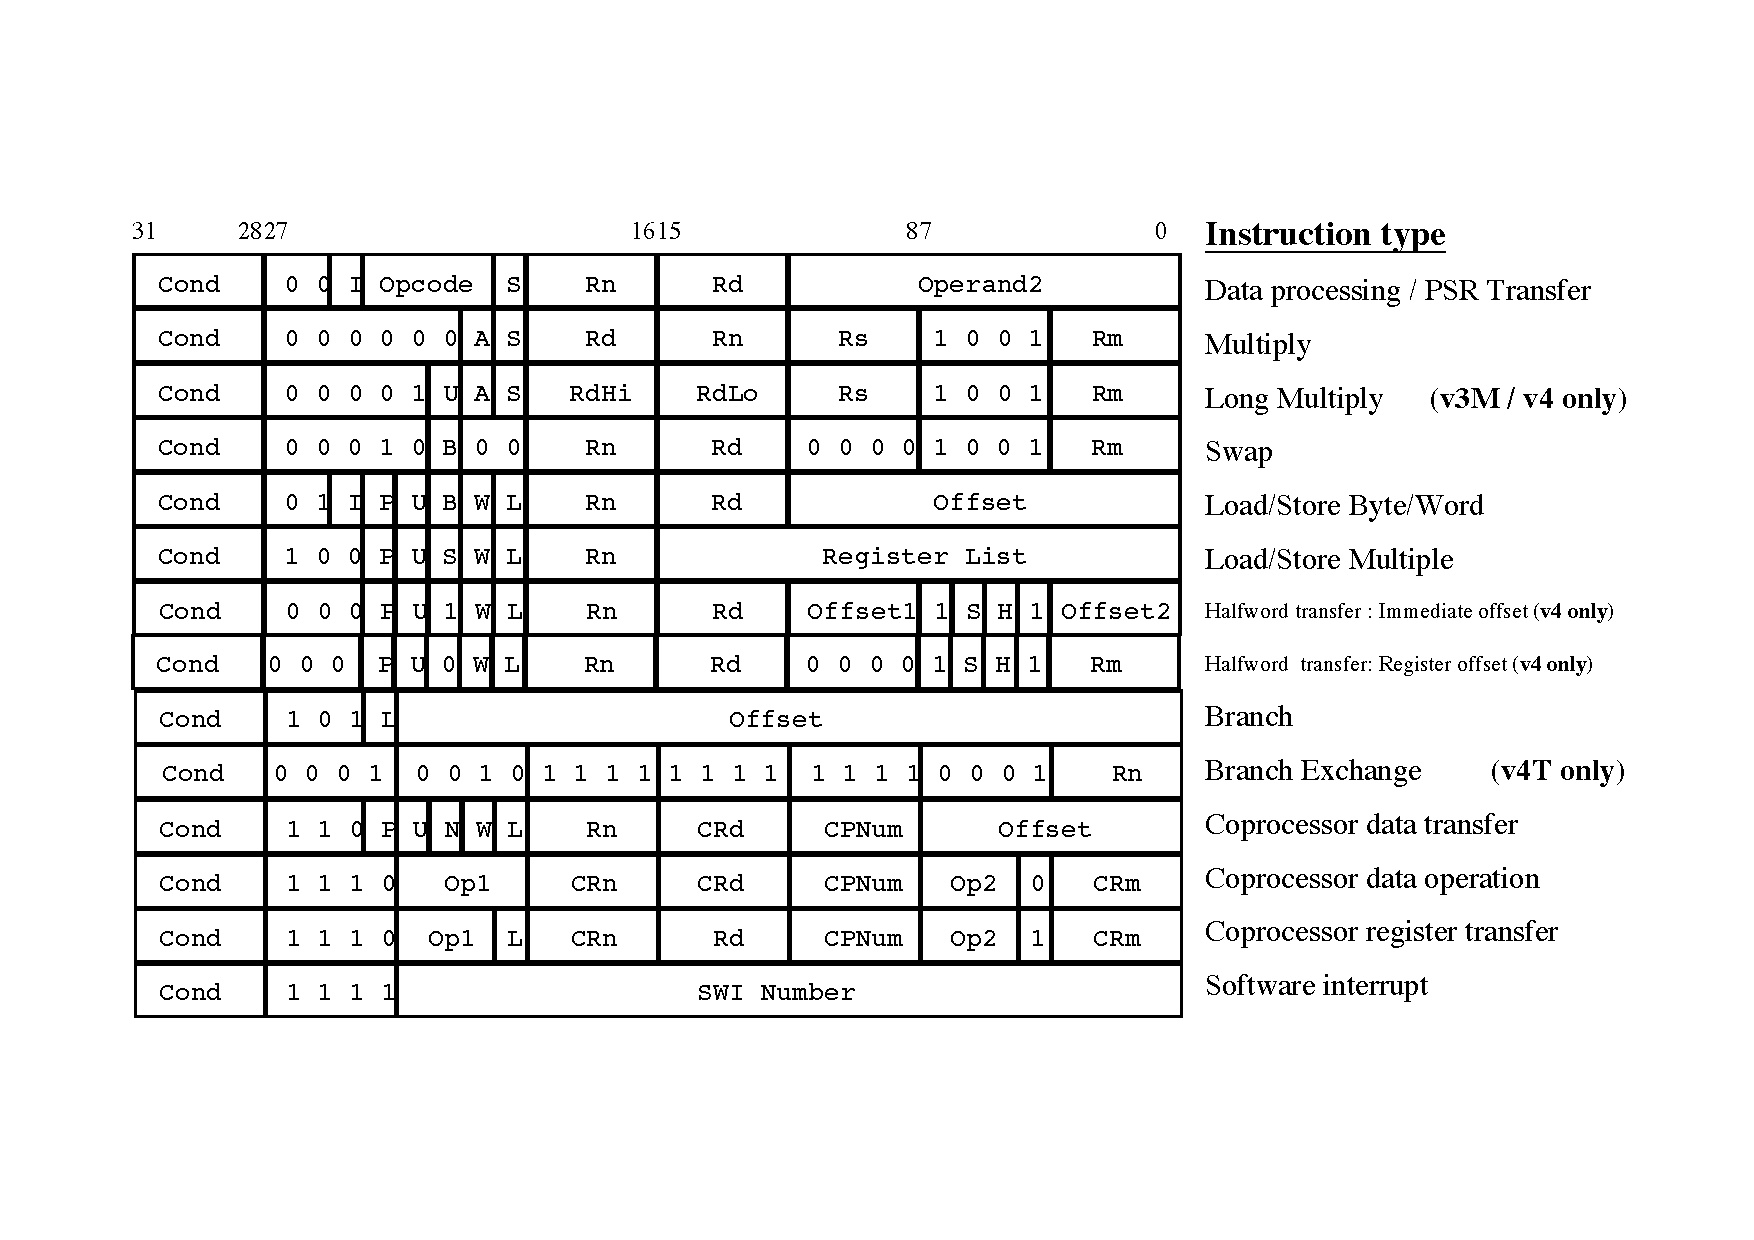
\includegraphics[width=1.0\textwidth]{./fig/InstructionFormat.pdf}
	\caption{ARM instruction set format from \cite[p. 13]{ARMInst}.}
	\label{fig:instructionformat}
\end{figure}

Thumb

ARM provides the \emph{Unified Assembler Language} (UAL) as a canonical language for all ARM and Thumb commands. Assembly written in UAL can be assembled to ARM alone, or to ARM with Thumb, depending on the target processor.

An interesting feature of ARM instructions is their conditional bits, which can be seen in Figure~\ref{fig:instructionformat} as bits 31--28. In UAL, ARM instructions that end in \texttt{S} (for example \texttt{ADDS} vs. \texttt{ADD}, and \texttt{SUBS} vs. \texttt{SUB}) set the condition flags in the APSR (bits 31--28). The value of these four bits together with the state of the condition flags in the APSR determine whether or not the instruction is executed. The different condition codes are listed in Figure~\ref{fig:conditioncodes}. Even if not executed the instruction still uses one cycle.

\begin{figure}[htb]
	\centering
	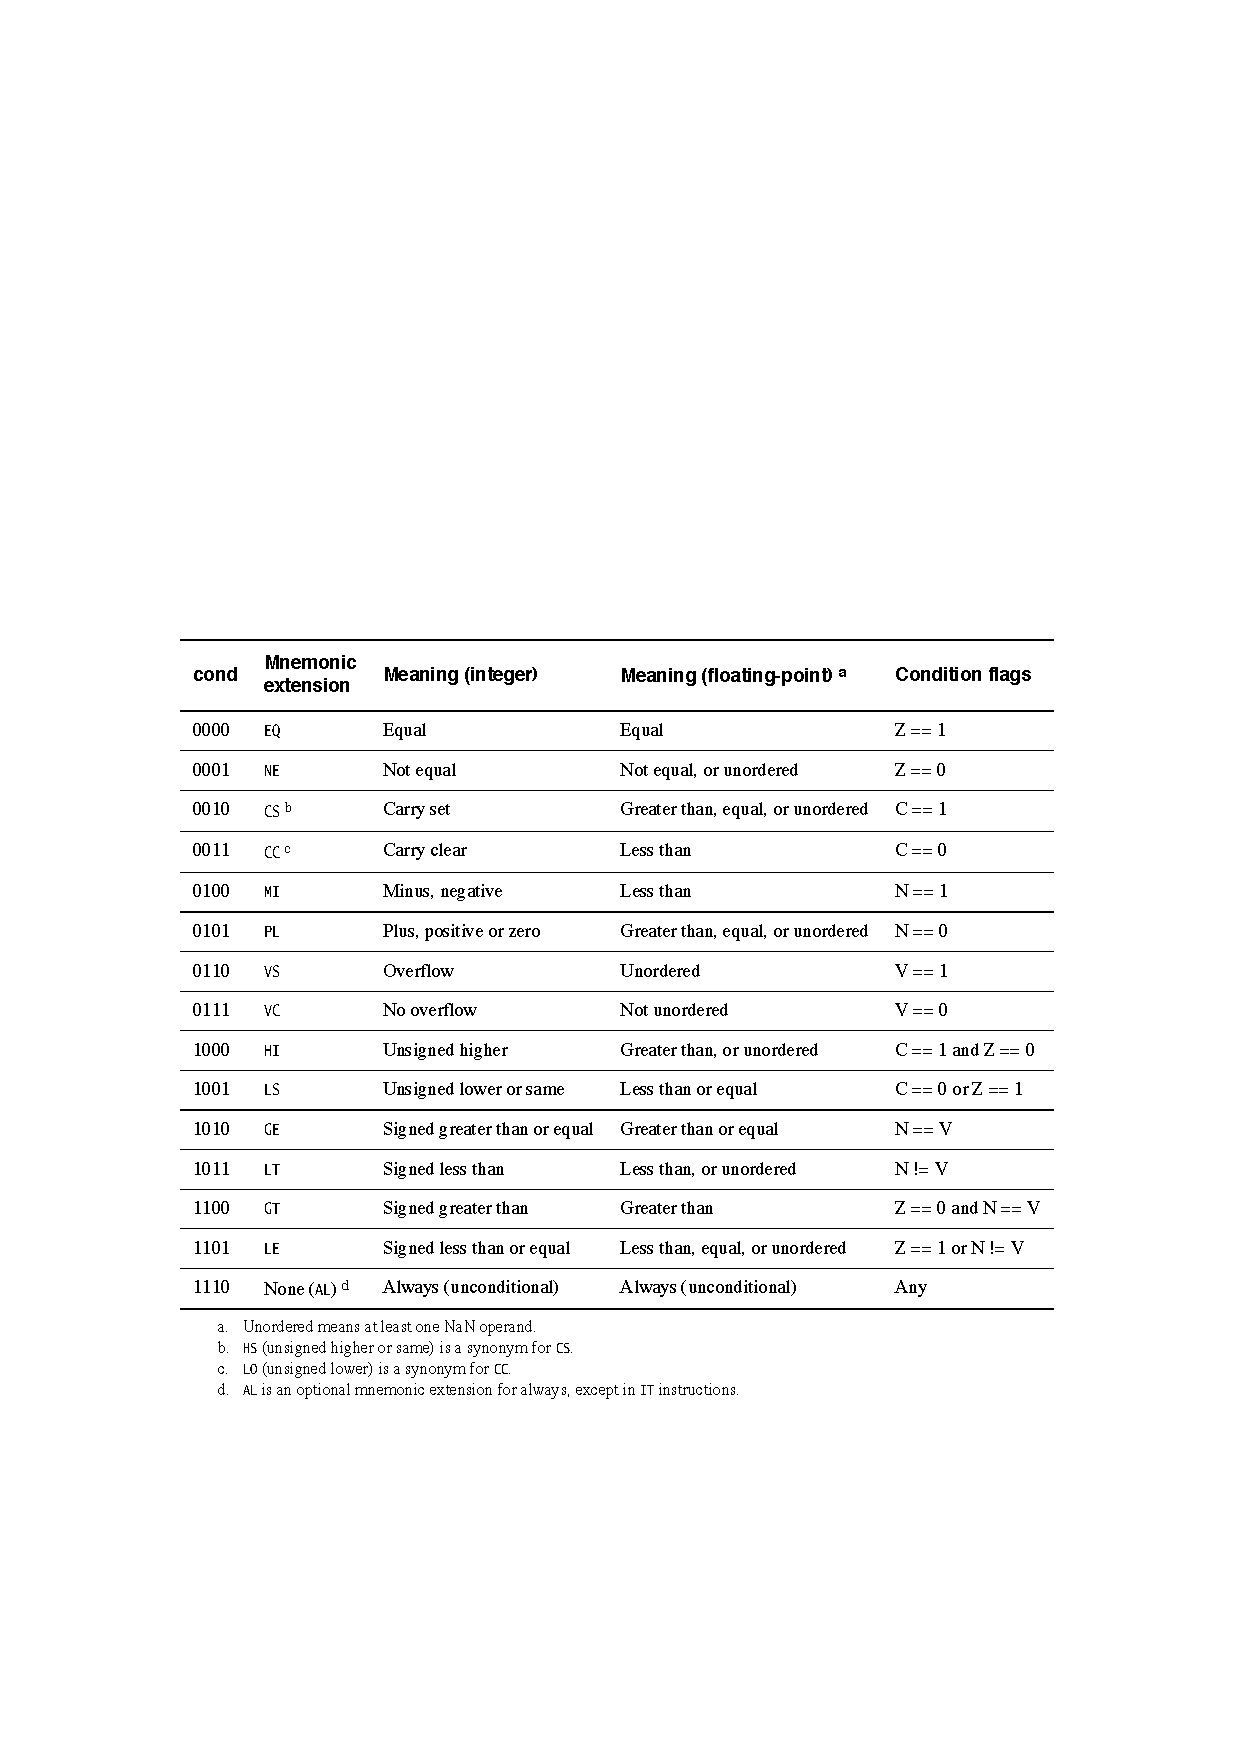
\includegraphics[width=1.0\textwidth]{./fig/ConditionCodes.pdf}
	\caption{Condition codes from \cite[p. A8-8]{ARMRef}.}
	\label{fig:conditioncodes}
\end{figure}

conditional instructions
APSR

A4
A5.1
Condition execution A8-8
\chapter{Unusual Instructions}
Perhaps in A4.4.6, A4.4.7, A4.8
bit fields?
\chapter{Memory Management}
A3
B2

6-2
\chapter{ARM Assembly Example}
iOS ABI Function Call Guide \cite{iOSABI}

\begin{figure}[htb]
	\centering
	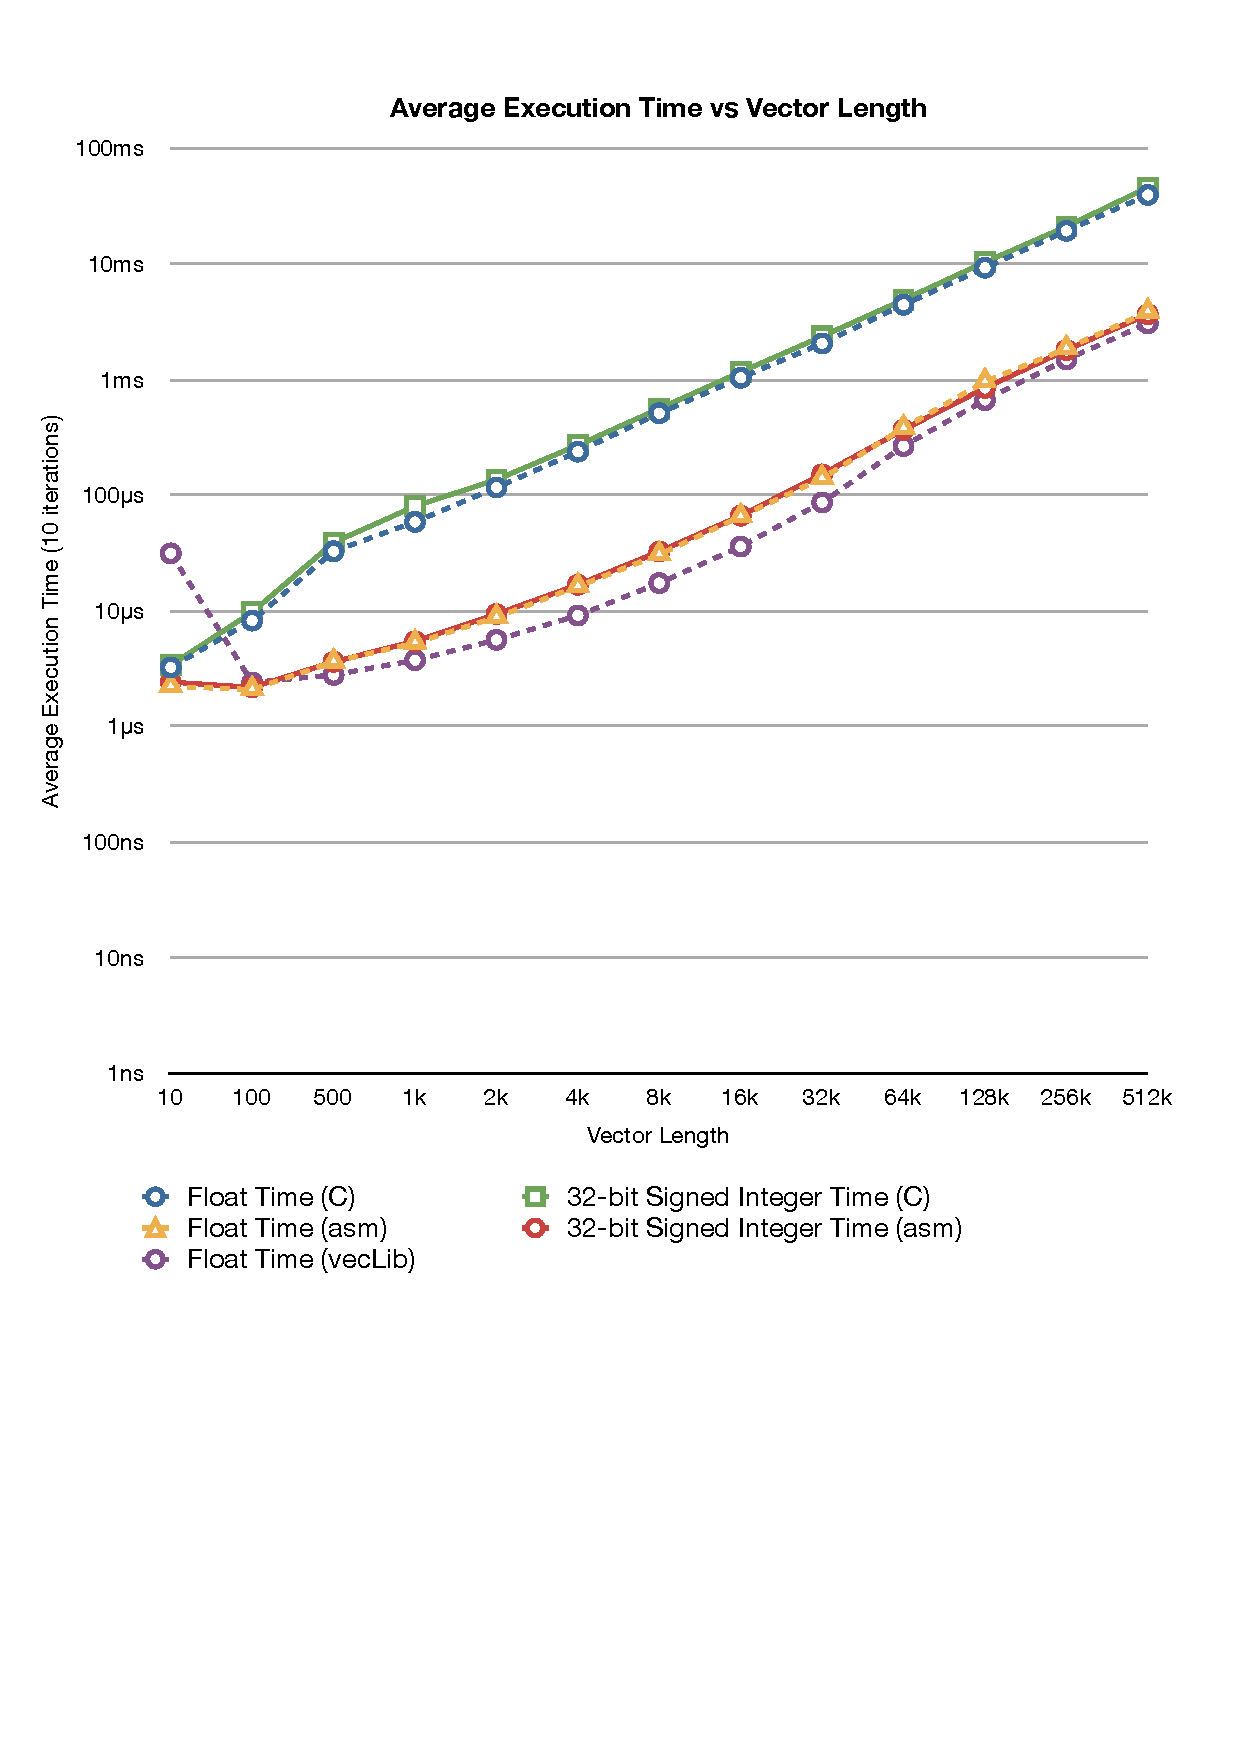
\includegraphics[width=1.0\textwidth]{./fig/ResultsChart.pdf}
	\caption{\ldots}
	\label{fig:results}
\end{figure}

\begin{table}[htb]
	\centering
	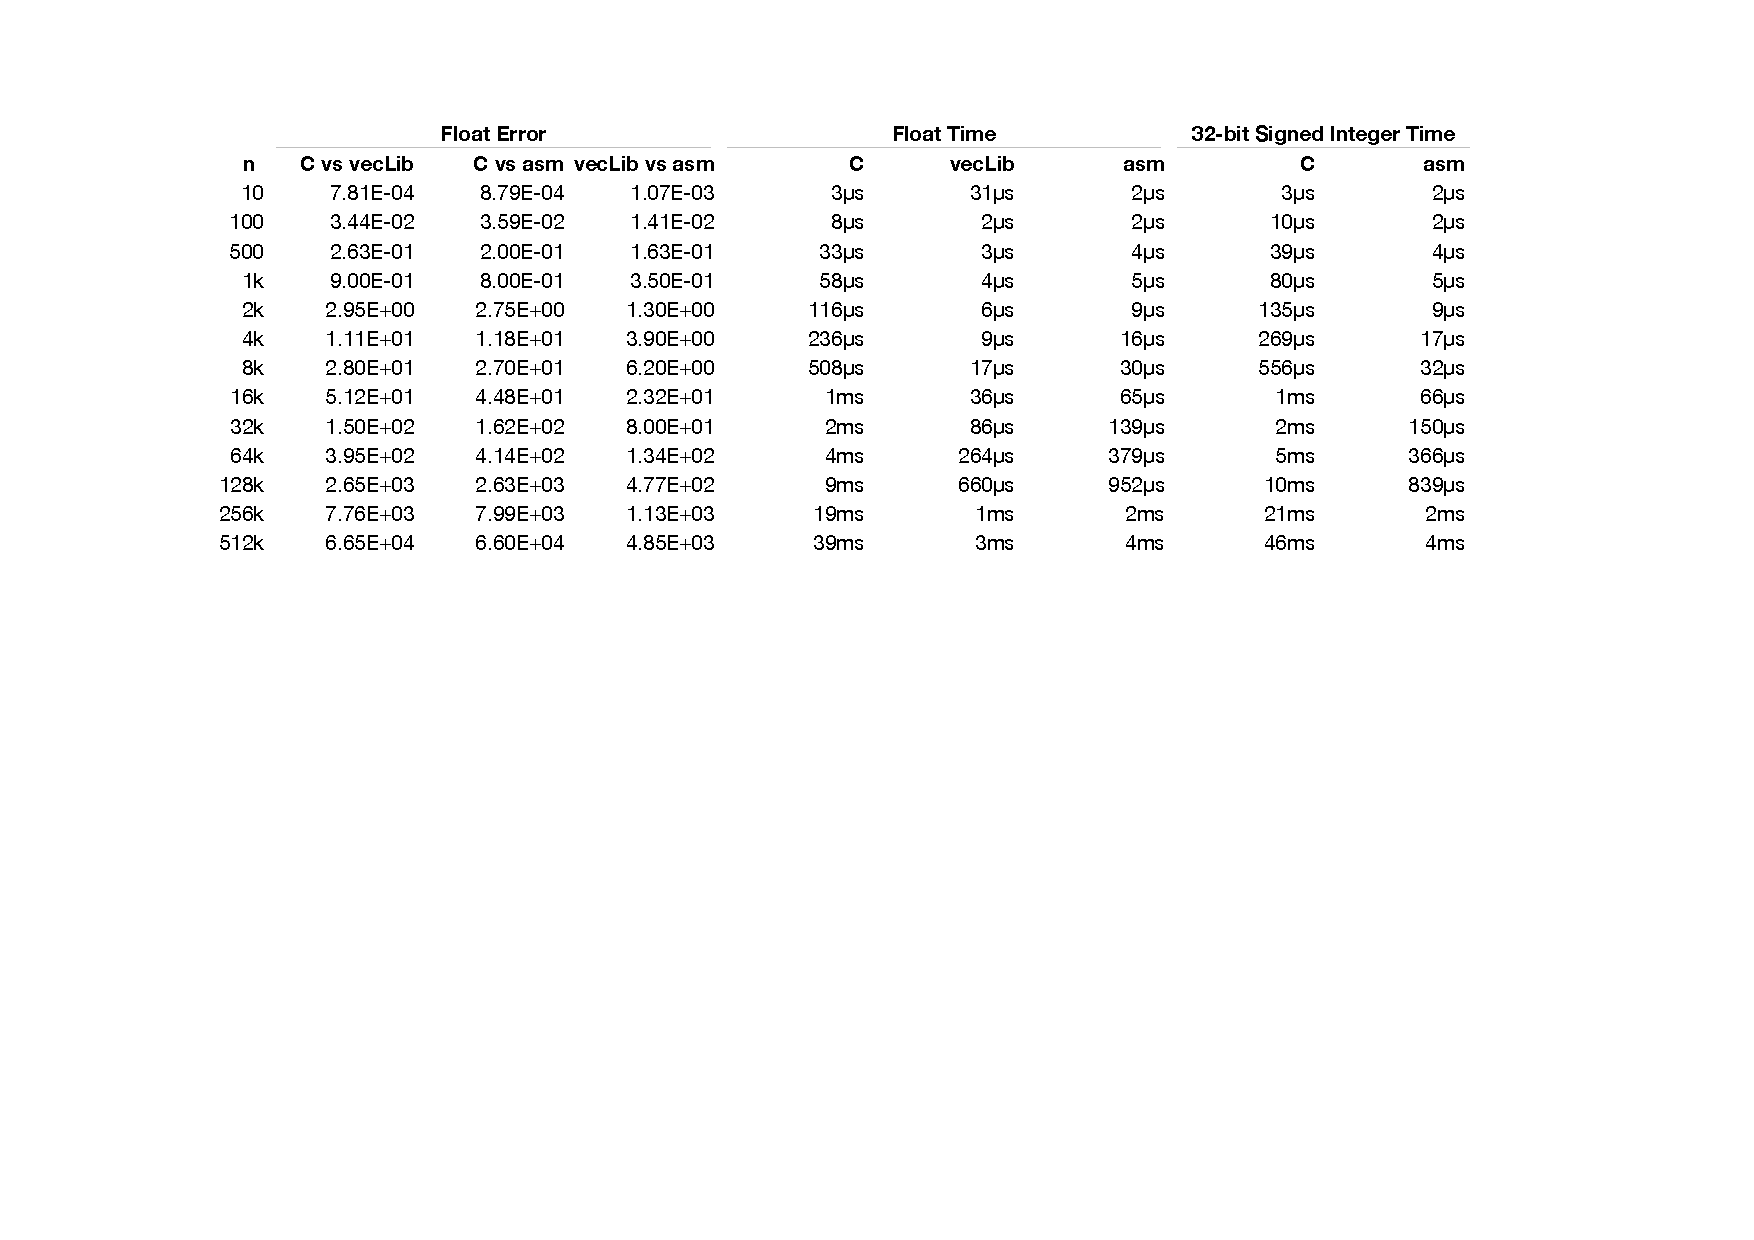
\includegraphics[width=1.0\textwidth]{./fig/ResultsTable.pdf}
	\caption{\ldots}
	\label{tab:results}
\end{table}

\bibliographystyle{plain}
\bibliography{ARM_Report}

\clearpage

\appendix
\chapter{ARM Assembly Programming Example -- Inner Product of Two Vectors}

\begin{singlespacing}
\lstinputlisting[language={[ARM]Assembler}]{../ARM/dot_product.s}	
\end{singlespacing}  

\end{document}
